\normaltrue \difficilefalse \tdifficilefalse
\correctionfalse

%\UPSTIidClasse{11} % 11 sup, 12 spé
%\newcommand{\UPSTIidClasse}{12}

\exer{Vilebrequin $\star$ \label{B2:14:1023}}
\setcounter{question}{0}\UPSTIcompetence[2]{B2-14}
\index{Compétence B2-14}
\index{Vilebrequin}
\index{Centre de gravité}
\index{Centre d'inertie}
\ifcorrection
\else
\textbf{Pas de corrigé pour cet exercice.}
\fi



\ifprof
\else

Soit le vilebrequin représenté sur la figure suivante. On suppose que sa masse volumique $\mu$ est constante. 
Par ailleurs l'accélération de la pesanteur est portée par $-\vect{y}$ : $\vect{g} = -g\vect{y}$.
\begin{figure}[H]
\centering
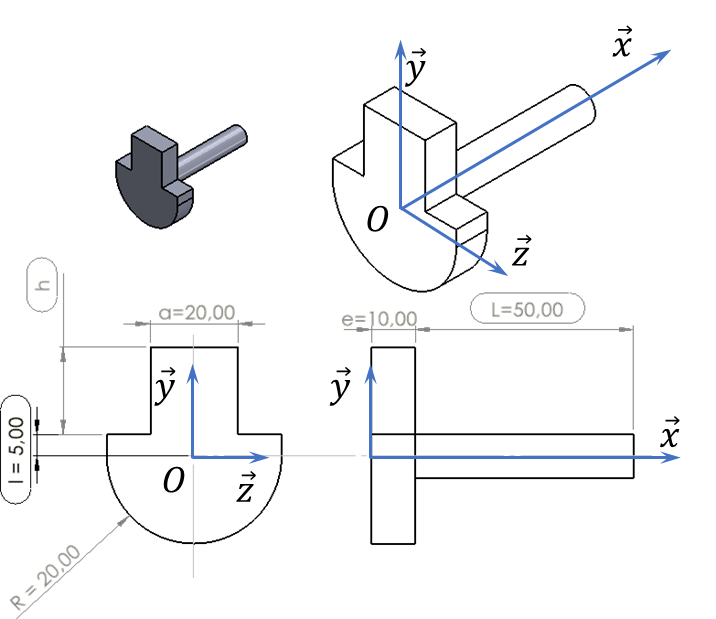
\includegraphics[width=\linewidth]{1023_03}
\end{figure}
\fi



\question{Exprimer sous forme littérale l'expression de la position du centre d'inertie du solide.}
\ifprof
\else
\fi


\question{Déterminer $h$ pour que le centre d'inertie appartienne à l'axe de rotation $\axe{O}{x}$ du vilebrequin.}
\ifprof
\else
\fi


\question{Faire l'application numérique.}
\ifprof
\else
\fi


\question{Exprimer le torseur de pesanteur sur le vilebrequin en $G$ puis en $O$.}
\ifprof
\else
\fi



\ifprof
\else
\begin{flushright}
\footnotesize{Corrigé  voir \ref{B2:14:1023}.}
\end{flushright}%
\fi